\documentclass{article}

% Language setting
% Replace `english' with e.g. `spanish' to change the document language
\usepackage[english,russian]{babel}
\usepackage{amsmath}

%графика
\usepackage{wrapfig}
\usepackage{graphicx}
\usepackage{pgfplots}
\usepackage{tikz}


\usepackage{tcolorbox}

% Set page size and margins
% Replace `letterpaper' with `a4paper' for UK/EU standard size
\usepackage[letterpaper,top=2cm,bottom=2cm,left=3cm,right=3cm,marginparwidth=1.75cm]{geometry}

% Useful packages
\usepackage{amsmath}
\usepackage{amssymb}
\usepackage{graphicx}
\usepackage{fixltx2e}
\usepackage[colorlinks=true, allcolors=blue]{hyperref}

\usepackage{geometry}
\geometry{left=25mm,right=25mm,
 top=25mm,bottom=25mm}

\title{Quantitative Analytics.\\
Lectures. Week 3. \\
Modeling Non Parallel Term Structure Shifts and Hedging. Моделирование непараллельных сдвигов временной структуры и хеджирование.}
\author{Kamenskaya Elizaveta}

% Колонтитулы
\usepackage{fancyhdr}
\pagestyle{fancy}
\renewcommand{\headrulewidth}{0.1mm}  
\renewcommand{\footrulewidth}{0.1mm}
\lfoot{}
\rfoot{\thepage}
\cfoot{}
\rhead{CMF-2022}
\chead{}

\begin{document}
\maketitle

% Оглавление
\setcounter{tocdepth}{1} % {2} - в оглавлении участвуют chapter, section и subsection. {1} - только chapter и section
\renewcommand\contentsname{Contents}
\tableofcontents
\newpage

% \section{Dictionary, Definitions, Abbreviations}

% \subsection{Dictionary}
% \begin{itemize}
%     \item IR - Interest rate - процентная ставка.
%     \item Compounding - платежи (idk)
% \end{itemize}

% \subsection{Definitions and Abbreviations}
% \begin{itemize}
%     \item SAR - Stated annual rate.
%     \item EAR - Effective annual rate.
%     \item FoC - Frequency of Compounding
%     \item PMT - Payment
%     \item r - Interest rate (at the moment). 
% \end{itemize}

\renewcommand{\labelitemi}{\tiny$\bullet$}
\renewcommand{\figurename}{Fig.}

 \section{Weaknesses of single-factor approaches}
 \begin{itemize}
     \item A single-factor approach assumes that within the term structure of interest rates (yield curve) all rate changes are driven by a single factor (shifts are parallel).

     \item The yield curve risk exists - a risk rates along the term structure move differently. Single-factor approach has no protection against that.
 \end{itemize}


\section{Principal Components Analysis}

\textbf{Principal Components Analysis} - a statistical technique that can be used to understand term structure movements in historical data.

It looks at daily movements in rates and identifies the underlying factors that affect those movements.

Requirements:
\begin{itemize}
    \item Term structure movements (movements of every rate) are a linear combination of the factors.

    \item Factors are uncorrelated

    \item Most significant 2-3 factors account for most of the daily movements
\end{itemize}

\begin{center}
    FACTORS =/= RATES
    
    But number of factors = number of rates

    (otherwise it will be unsolvable)
\end{center}

\begin{figure}[h]
\centering
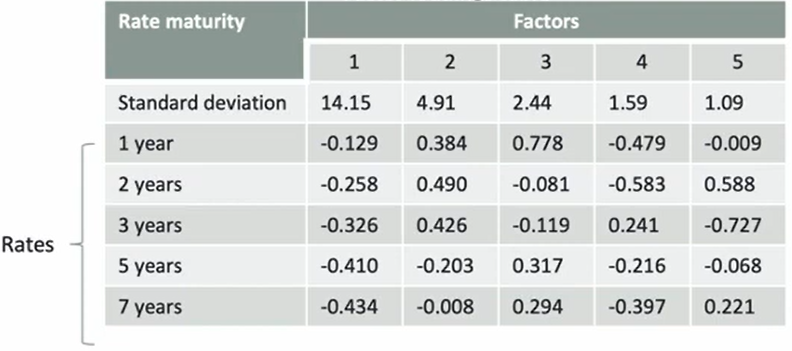
\includegraphics[width=0.7\textwidth]{factor loadings table.png}
\caption{Factor loadings table}
\label{loadings}
\end{figure}

Change in j-th rate: $\sum_{i=1}^{5} a_i f_{ij}$ :
\begin{itemize}
    \item $a_i$ - factor score - observed realization of i-th factor

    \item $f_{ij}$ - factor loading

    \item The importance of a factor is measured by the standard deviation of its factor scores
\end{itemize}

Based on the data in Fig. 1:
\begin{itemize}
    \item When there is +1 unit of Factor 1, the one-year rate changes by -0.129 basis points, the two-year rate changes by -0.258 basis points, and so on

    \item $\frac{14.15^2 + 4.91^2 + 2.44^2}{14.15^2 + 4.91^2 + 2.44^2 + 1.59^2 + 1.09^2} = 98.4\%$ of variance explained by first 3 factors

    \item Factor 1 moves all rates in the same direction - general movement

    \item Factor 2 moves short-term and long-term in different directions

    \item Factor 3 is a bowing of the term structure
\end{itemize}


\section{Key rate shifts and partial '01s}

\textbf{Key rate exposures} help describe how the risk of a bond portfolio is distributed along the term structure, and they assist in setting up a proper hedge for a \textbf{bond portfolio}.
They are utilized for measuring and hedging risk in bond portfolios using rates from the most liquid bonds available (usually government, recently issued, near par).

\textbf{Key rate shift technique} is an approach to nonparallel shifts in yield curve, which allows for changes in all rates to be determined by changes from selected key rates.

Simplifying assumption: \textbf{all rates can be determined as a function of a few "key rates"}.

Small number of key rates are used - most liquid government securities.

Most common key rates - par yield bonds - 2-,5-,10- and 30-year.

\textbf{Key rate shift} - one basis point shift of one of those rates.

Changes in each key rate affect rates from the term of \textbf{the previous key rate to the term of the subsequent key rate.}

This technique can be applied to both \textbf{spot rates} and \textbf{par rates}.

\begin{wrapfigure}{r}{0.4\textwidth}
    \centering    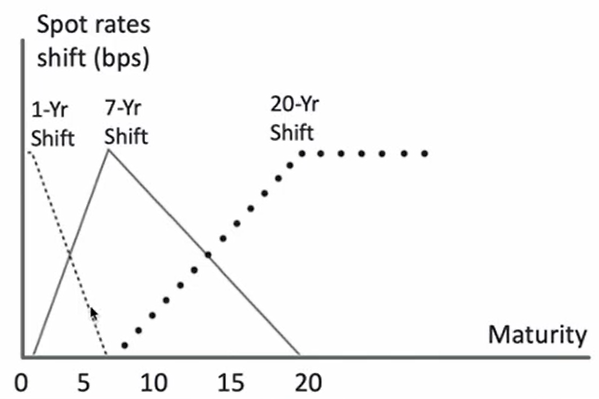
\includegraphics[width=0.4\textwidth]{rates.png}
\end{wrapfigure}

\underline{Example: Key rates}
\begin{itemize}
    \item 1-year rate will affect all rates from 0 to 7

    \item 7-year rate will affect all rates from 1 to 20

    \item 20-year rate will affect all rates from 7
\end{itemize}

The combined of the three key rate shifts is a one-basis point shift in all rates.

The impact of key rate shifts are sometimes referred to as \textit{partial '01s} or \textit{key rate '01s} (KR01s).

\underline{Example: Key rate partial '01s and durations}

\begin{figure}[h]
    \centering    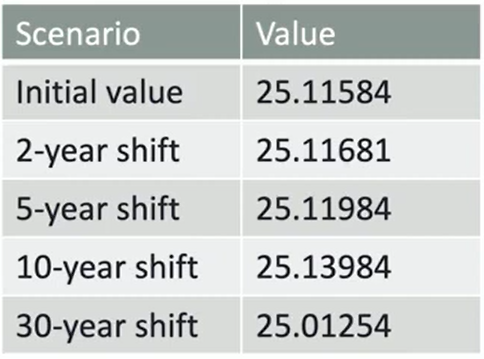
\includegraphics[width=0.3\textwidth]{kr01.png}
\end{figure}


\begin{align*}
    '01_{5-year} &= -\frac{25.11984 - 25.11584}{10 000 * 0.0001} = -0.004
    \\
    D_{5-year} &= -\frac{25.11984 - 25.11584}{25.11584 * 0.0001} = -1.59
\end{align*}
    
\begin{itemize}
    \item Unlike in single-factor model, partial '01s and duration here only correspond to the particular key rate and its vicinity, not all rates

    \item Summing all 4 durations would provide us with the effective duration

    \item $DV01 = DV01_{2-year} + DV01_{5-year} + DV01_{30-year}$ 
\end{itemize}

\newpage

\section{Hedging applications}

\underline{Example: Hedging based on key rates}

Suppose a 30-year semiannual-paying non-callable bond that pays a 4500 semiannual coupon in a flat rate environment of 5\% across all maturities.

\begin{figure}[h]
    \centering    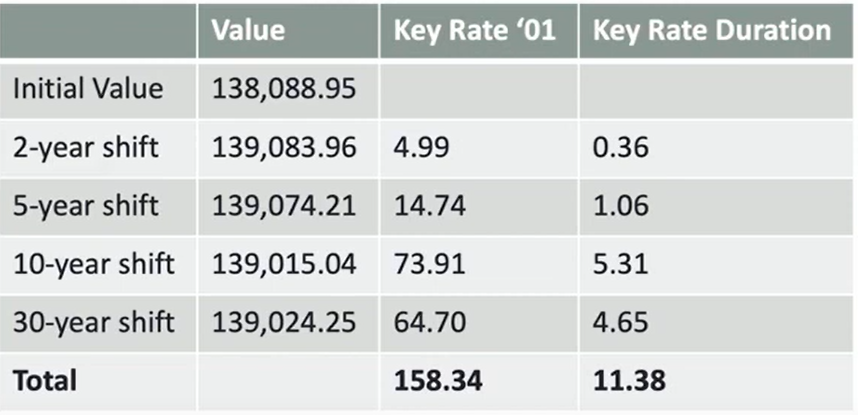
\includegraphics[width=0.6\textwidth]{hedging.png}
\end{figure}

\begin{itemize}
    \item A 2-year security only has a 2-year key rate exposure of 0.015 per \$100 face value.

    \item A 5-year security has exposures over the 2-year and 5-year key rate of 0.0025 and 0.035, respectively, per \$100 face value.

    \item A 10-year security has exposures over the 2-year, 5-year and 10-year key rates of 0.003, 0.015 and 0.1, respectively, per \$100 face value.
    
    \item A 30-year security only has exposure to the 30-year key rate of 0.15 per \$100 face value.
    
\end{itemize}
\begin{equation*}
    \left\{\begin{matrix}
    \frac{0.015}{100} \times F_2 + \frac{0.0025}{100} \times F_5 + \frac{0.003}{100} \times F_{10} = 4.99
    \\
    \frac{0.035}{100} \times F_5 + \frac{0.015}{100} \times F_{10} = 14.74
    \\
    \frac{0.1}{100} \times F_{10} = 73.91
    \\
    \frac{0.15}{100} \times F_{30} = 64.70
\end{matrix}\right.

\end{equation*}

\begin{center}
To get rid of sensitivity to each key rate, we need to short:
\begin{align*}
    F_2 &= 16.745
    \\
    F_5 &= 10.439
    \\
    F_{10} &= 73.910
    \\
    F_{30} &= 43.133    
\end{align*}
\end{center}

\section{Bucketing approach}

\begin{wrapfigure}{r}{0.4\textwidth}
    \centering    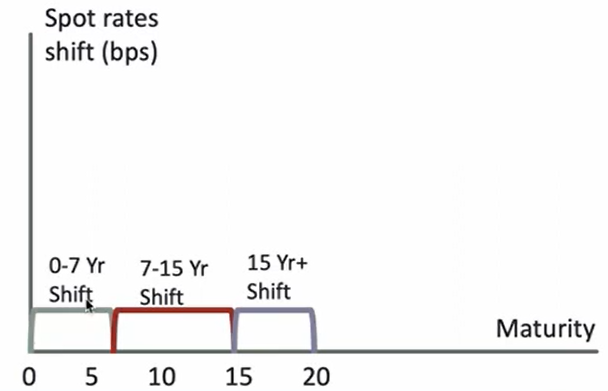
\includegraphics[width=0.4\textwidth]{buckets.png}
\end{wrapfigure}

A variation on the key rate shifts approach is to divide the interest rate term into segments referred to as buckets, and then calculate the dollar impact of changing all the spot rates in a bucket by one basis point on the value of a portfolio.

\textbf{Forward-bucket '01s} are computed by shifting the forward rate over several regions of the term structure, one region at a time, after the term structure is divided into various buckets.

This technique can be applied to both \textbf{spot rates} and \textbf{forward rates}.

The approach is similar to key rates, but shifts are defined differently.

\underline{Example:}

\begin{figure}[h]
    \centering    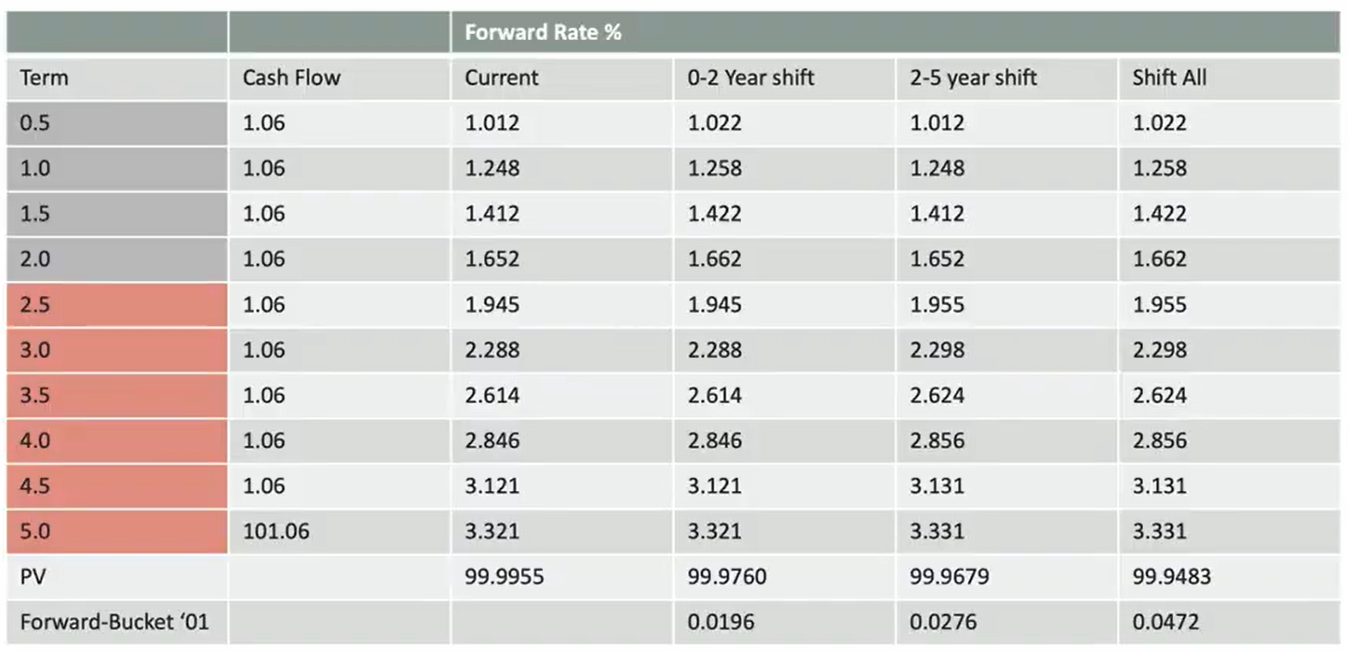
\includegraphics[width=0.9\textwidth]{partial.png}
\end{figure}

We have divided terms into two buckets: 0.5 to 2 and 2.5 to 5. Now we shift rates one bucket at a time and calculate new bond price (PV). Using the DV01 formula we can find the sensitivity of the price to the shift in each bucket (Forward-Bucket '01s). The last column is the result of single-factor approach.

\section{Estimating portfolio volatility}

These multi-factor approaches work well not only on estimating changes in the level of the portfolio, but also the estimation of portfolio volatility because it incorporates correlation effects between various interest rate assumptions.

Suppose one has information related to the volatility effects of two key rates. The traditional portfolio volatility relationships can be used not only to incorporate the volatility impacts of each rate, but also to incorporate correlation between them.

\end{document}
